% Chapter 1

\chapter{Thiết kế cơ sở dữ liệu} % Main chapter title

\label{Chapter5}
Dữ liệu thu thập được từ Smart BK Traffic và crowdsourcing cần phải được lưu trữ để tiến hành mining và cung cấp cho người dùng. Do đó hệ cơ sở dữ liệu cần phải đáp ứng được các nhu cầu:
\begin{itemize}
    \item Khả năng lưu trữ lượng dữ liệu lớn.
    \item Đáp ứng được nhu cầu lưu trữ từ nhiều nguồn thông tin khác nhau.
    \item Truy xuất và xử lý nhanh chóng, chính xác.
\end{itemize}
Dữ liệu thông thường được lưu trữ trên các hệ cơ sở dữ liệu NoSQL, mà cụ thể là MongoDB.

\section{MongoDB}
MongoDB là một cơ sở dữ liệu đa nền tảng, hoạt động dựa trên các khái niệm Collection và Document. Dữ liệu được lưu trữ dưới dạng các tài liệu JSON, cung cấp hiệu suất cao, khả năng truy xuất cao và mở rộng dễ dàng \cite{MongoDB1}.

\begin{figure}[H]
\centering
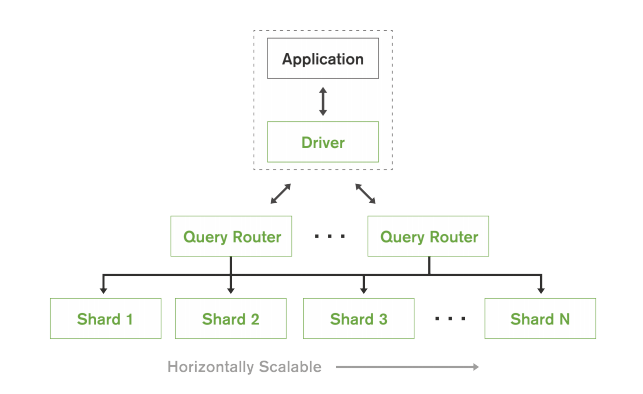
\includegraphics[width=0.8\textwidth]{Traffic_Report/images/image02.png}
\caption{Kiến trúc cơ sở dữ liệu MongoDB}\label{}
\end{figure}

Cách thức hoạt động của MongoDB:
\begin{itemize}
    \item MongoDB hoạt động dưới một tiến trình ngầm service, với cổng mặc định là 27017 để lắng nghe các sự kiện gửi từ ứng dụng rồi tiến hành xử lý.
    \item Mỗi document (bản ghi) được định danh bằng trường \textit{\_id} có kiểu \textit{ObjectId}. Trường \textit{\_id} là duy nhất để phân biệt giữa các bản ghi với nhau và để phục vụ các truy vấn dữ liệu. Nó được tự động đánh chỉ mục (index) để tốc độ truy vấn thông tin đạt hiệu suất cao nhất \cite{MongoDB2}.
    \item Khi có truy vấn dữ liệu, bản ghi được ghi đệm lên bộ nhớ RA, nhờ vậy các lượt truy vấn sau có tốc độ xử lý cao hơn thay vì lại đọc trực tiếp từ ổ cứng.
    \item Các truy vấn DML (thê, sửa, xoá) một bản ghi không được trực tiếp lưu ngay xuống ổ cứng, mà sau mỗi 60 giấy MongoDB mới tiến hành cập nhật toàn bộ dữ liệu thay đổi từ RAM xuống ổ cứng \cite{MongoDB3} nhằm đảm bảo hiệu suất của ứng dụng.
\end{itemize}

Ưu điểm khi sử dụng MongoDB:
\begin{itemize}
    \item MongoDB lưu trữ dữ liệu dưới dạng JSON nên dễ quản lý. Dữ liệu được mô tả tường minh, cấu trúc lại linh hoạt, dễ sử dụng cả về phía con người.
    \item Khả năng mở rộng lớn mà không cần lo lắng về các ràng buộc khoá chính, khoá ngoại...
    \item Dữ liệu khi truy vấn được lưu trữ trên RAM nên nâng cao tốc độ và hiệu suất của ứng dụng, nhất là đối với ứng dụng về giao thông cần lưu trữ và xử lý lượng dữ liệu rất lớn.
\end{itemize}

Bên cạnh đó, MongoDB cũng tồn tại một số nhược điểm như tốn nhiều bộ nhớ RAM, khả năng bị mất dữ liệu trong trường hợp đột xuất như mất điện, do MongoDB không lưu dữ liệu về ổ cứng ngay lập tức... 

Sau khi tìm hiểu, tổng kết lại các ưu và nhược điểm thì MongoDB là sự lựa chọn phù hợp để xây dựng cơ sở dữ liệu trong việc phát triển ứng dụng dự đoán giao thông.
\section{Mô hình quan hệ thực thể}
\section{Phân tích }